\documentclass[conference]{IEEEtran}

\IEEEoverridecommandlockouts

\usepackage{cite}
\usepackage{amsmath,amssymb,amsfonts}
\usepackage{algorithmic}
\usepackage{graphicx}
\usepackage{textcomp}
\usepackage{xcolor}

\usepackage{booktabs} %@{}
\usepackage{pgfplots}
\pgfplotsset{compat=1.16}
\usepackage[per-mode=symbol,detect-all]{siunitx}
\usepackage{hyperref}
\usepackage{cleveref} %\Cref{} vs. \cref{}
\usepackage[protrusion=true,expansion=true]{microtype}
\usepackage{mathabx} % for \bigtimes


\def\BibTeX{{\rm B\kern-.05em{\sc i\kern-.025em b}\kern-.08em
    T\kern-.1667em\lower.7ex\hbox{E}\kern-.125emX}}

\begin{document}


\title{\LARGE \textbf{Planning Under Uncertainty with Sensor Occlusions in \\ Urban Driving Scenarios} % \\
%\thanks{Ross Alexander is supported by a Stanford Graduate Fellowship (SGF) in Science and Engineering.}
}


\author{\IEEEauthorblockN{  Ross Alexander}
\IEEEauthorblockA{\textit{  Department of Aeronautics and Astronautics} \\
\textit{                    Stanford University} \\
                            Stanford, CA 94305 \\
                            rbalexan@stanford.edu}} % or ORCID


\maketitle

\begin{abstract}
    Safe and efficient autonomous driving in urban scenarios requires a policy that is responsive to uncertainty in the environment and sensors. Partial observability of the environment due to sensor occlusions has led to conservative manually-designed collision avoidance policies that are inefficient. Since collision avoidance is a sequential decision-making problem under uncertainty, it can be posed as a partially observable Markov decision process (POMDP), which can be solved to generate an optimal policy. We leverage the POMDP formulation to generate approximately optimal collision avoidance policies and evaluate the safety and efficiency of the resulting driving behaviors. We find that the policies outperform a random policy and are generally highly-performant and robust to uncertainty in the environment and sensors.
\end{abstract}

% \begin{IEEEkeywords}
% component, formatting, style, styling, insert
% \end{IEEEkeywords}

\section{Introduction}
\label{sec:introduction}

% Overview of topic sentences
Autonomous driving in urban scenarios requires navigating safely and efficiently in light of significant uncertainty presented by occlusions. In dense urban settings, buildings, signs, cars, and other physical obstacles frequently occlude other road users from the field of view of the sensors. Planning in these occluded scenarios requires judicious safety thresholds in order to ensure collision-free driving. In this paper, we focus on developing safe and efficient policies for collision avoidance while passing a crosswalk with pedestrians emerging from an occluded region.

% What is the problem?                     
We consider the occluded crosswalk scenario depicted in \Cref{fig:occluded_crosswalk_scenario}. The scenario consists of an autonomous vehicle driving along a roadway and a pedestrian crossing the roadway at a crosswalk. The ego vehicle's sensors are occluded by a static obstacle that prevents the pedestrian from being observed. 

\begin{figure}[htbp]
    \centerline{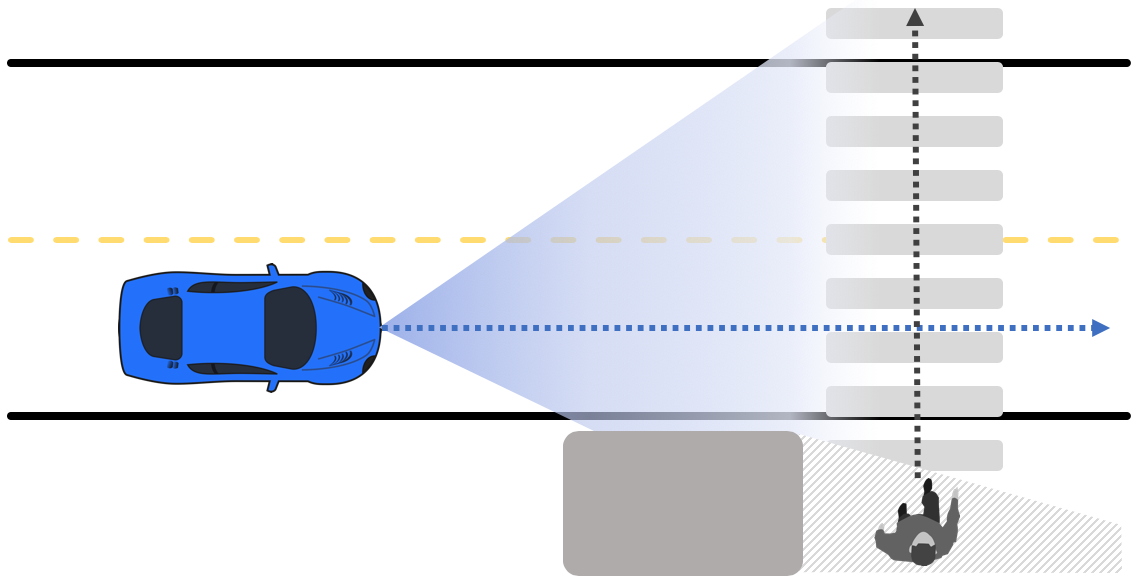
\includegraphics[width=0.95\linewidth]{doc/main/occluded_crosswalk_scenario.png}}
    \caption{The occluded crosswalk scenario. The ego vehicle (in blue) is driving along the roadway and the pedestrian (in gray) is crossing the crosswalk. The static obstacle occludes the ego vehicle's sensors and prevents observation of the pedestrian.}
    \label{fig:occluded_crosswalk_scenario}
\end{figure}

% Why is it interesting and important?
% Why is it hard? Why do naive approaches fail?
Urban driving scenarios are often heavily occluded, which presents significant challenges in achieving fully autonomous driving. Occlusions in urban scenarios can arise as a result of \textit{static obstacles}, such as buildings, signs, and parked cars, but can also arise as a result of \textit{dynamic obstacles}, such as moving pedestrians and moving cars. Above all, the autonomous vehicle must navigate safely and avoid collision with pedestrians. However, the autonomous vehicle must also navigate efficiently and cannot be paralyzed by the significant uncertainty in the environment and sensors. A pedestrian's pose and velocity may be completely unobservable due to a sensor occlusion, or at best, partially observable due to sensor uncertainty. As a result, the occluded crosswalk scenario strongly captures the trade-off between safety and efficiency in autonomous driving. Optimizing this trade-off and generating a driving policy that is safe and robust to uncertainty in the environment and sensors is a critical step in urban autonomous driving.

% Why hasn't it been solved before? (Or, what's wrong with previous proposed solutions? How does mine differ?)
Planning in occluded scenarios faces two main challenges. First, the planning algorithm must be able to handle partial observability. Planning requires not only reasoning about an unoccluded pedestrian's pose and velocity, which can only be observed with finite accuracy and precision, but also reasoning about a potentially occluded pedestrian's pose and velocity, which cannot be observed. And second, real urban driving scenarios often contain multiple road users. While solving the occluded crosswalk problem with a single road user can be useful in theory, it is hardly useful in practice. Unfortunately, solving the occluded crosswalk problem with multiple road users can be intractable for many planning algorithms. Thus, a solution for planning in occluded scenarios must be capable of simultaneously handling partial observability of multiple road users in a way that maintains safety and efficiency, and finally, in a way that respects real-time decision-making constraints.

% What are the key components of my approach and results? Also include any specific limitations.
In this paper, we consider the problem of avoiding collisions with pedestrians crossing behind an occluded region on the side of the road and attempt to recreate and extend the results in \cite{Bouton2018ScalableDriving}. The approach formulates the multiple road user collision avoidance problem as a partially observable Markov decision process (POMDP) with discrete state, action, and observation spaces. The POMDP is solved using offline techniques to obtain driving policies, which are evaluated in simulation and compared against a random policy on safety and efficiency metrics. 

% Summary of the major contributions in bullet form, mentioning in which sections they can be found. This material doubles as an outline of the rest of the paper, saving space and eliminating redundancy.
We discuss related work in \Cref{sec:related-work} and describe the partially-observable Markov decision process (POMDP) and solution techniques for generating an approximately optimal policy in \Cref{sec:background}. \Cref{sec:proposed-approach} discusses how the collision avoidance problem can be posed as a POMDP and the solution approaches we take in obtaining an approximately optimal policy. \Cref{sec:experiments-results} covers the experimental setup, analysis of the safety and efficiency criteria, and discussion of the resulting driving policies. Finally, we present our conclusions in \Cref{sec:conclusion} and provide some areas for further research in \Cref{sec:future-work}.


\section{Related Work}
\label{sec:related-work}

% Other planning frameworks
Several planning algorithms ensure collision-free paths when passing occluded regions. If objects emerging from occluded regions have a specified maximum velocity, the autonomous vehicle can follow a maximal velocity profile along its original planned path that ensures a collision-free trajectory \cite{Alami2002OnPlans}. Some approaches rely on the time-to-collision (TTC) metric and extensions of the TTC metric, which have shown to be reliable safety measures not only for vehicle collision avoidance, but also for pedestrian collision avoidance \cite{Minderhoud2001ExtendedAssessment, Volz2019InferringCrosswalks}. Many of these planning frameworks are designed solely around the use of \textit{autonomous emergency braking} (AEB) systems to perform drastic collision avoidance maneuvers. While AEB system planning frameworks are effective at ensuring essentially collision-free driving, they suffer from uncertainty in the environment and sensors that can create inefficient control policies likely to initiate unnecessary severe rapid braking.

% Modeling as a POMDP - single user
In order to develop driving policies robust to uncertainty in the environment and sensors, others have chosen to model the collision avoidance problem as a partially observable Markov decision process (POMDP). POMDPs have been used to successfully generate autonomous driving policies in occluded scenarios. In particular, several approaches have leveraged POMDPs to develop longitudinal-control policies for unsignalized intersections \cite{Brechtel2014ProbabilisticPOMDPs, Hubmann2019AScenarios} and for unsignalized crosswalks \cite{Thornton2018ValuePlanning, Thornton2019TowardValues, Kapania2019ACrosswalks}. Most of these approaches considered only one road user due to the increased algorithmic and computational complexity of considering multiple road users. While these approaches generated progress, their applicability is still limited since most urban scenarios contain multiple road users which limits their practical use.

% Modeling as a POMDP - multiple users
A scalable approach to avoiding multiple road users in both the unsignalized intersection and unsignalized crosswalk was achieved through utility fusion \cite{Bouton2018ScalableDriving}. The multiple road user collision avoidance problem was decomposed into single road user collision avoidance sub-problems enabling solution of the problem that scales linearly with the number of road users considered. The set of single road user optimal belief action utilities were synthesized to generate an approximation to the optimal belief action utility for all road users using a fusion function. The authors consider both sum and minimum fusion functions and find the minimum fusion function generates a more conservative policy. Others have expanded on the success of scalable longitudinal-control policies and developed scalable in-lane coupled longitudinal- and lateral-control policies augmented with AEB systems that maintain safety and improve scenario crossing speeds \cite{Schratter2019PedestrianOcclusions}.

% expanding to multiple road users
%-- the so-called "full-stop."


\section{Background}
\label{sec:background}

A principled and general framework for planning under uncertainty is the partially-observable Markov decision process (POMDP). A POMDP is defined by the tuple $\langle \mathcal{S},\mathcal{A}, \mathcal{O}, T, R, O, \gamma \rangle$, where $\mathcal{S}$ is the state space, $\mathcal{A}$ is the action space, $\mathcal{O}$ is the observation space, $T$ is the transition model, $R$ is the reward model, $O$ is the observation model, and $\gamma$ is the discount factor. A POMDP models the process where an agent in state $s \in \mathcal{S}$ takes action $a \in \mathcal{A}$ and transitions to a state $s' \in \mathcal{S}$ with probability $T(s, a, s') = \textnormal{Pr}(s' \mid s, a)$. Then, the agent observes $o \in \mathcal{O}$ with probability $O(o, s',a) = \textnormal{Pr}(o\mid s', a)$ and receives a real-valued reward $r = R(s, a)$. Rewards in the future are discounted by a factor $\gamma \in (0,1)$, so that immediate rewards are valued more than future rewards.

In a POMDP, the state of the environment may not be fully observable, so the agent maintains a belief $b$ about the underlying state, which is assumed to be a sufficient statistic for the agent's history of actions and observations. A belief is a categorical probability distribution over the state space that represents the probability of each state being the true underlying state. The belief $b$ is updated after taking action $a$ and observing $o$ using the Bayesian belief update:

\begin{equation}
    b'(s')~\propto~O(o \mid s', a) \sum_{s \in S} T(s' \mid s, a) b(s)
\end{equation}

% QMDP, SARSOP, and other solvers + brief descriptions
The solution to a POMDP is an optimal policy $\pi^*$ that maps beliefs to actions. Following the optimal policy from any initial state maximizes the expected discounted sum of future rewards. Computing the exactly optimal policy is generally intractable in non-trivial POMDPs, so we must use approximation techniques to compute an approximately optimal policy \cite{Madani2003OnProblems}. There are a variety of approaches for generating approximately optimal policies that can be broadly split into two classes: offline methods and online methods \cite{Kochenderfer2015DecisionApplication}. Offline approaches involve computing the entire policy prior to execution, which is typically computationally expensive. Online approaches involve computing a policy from the current belief state over a specified planning horizon. Online approaches benefit from the ability to plan over the reachable belief space, which is typically a small subspace of the entire belief space, but suffer from reduced computational budget due to real-time, finite-memory computational constraints.


\section{Proposed Approach}
\label{sec:proposed-approach}

\subsection{POMDP Model}

We describe in the following subsections how the single user occluded crosswalk problem can be formulated as a POMDP.

\subsubsection{Environment and initial conditions}
The roadway is $32 ~\si{\meter}$ long and crosswalk is located $20 ~\si{\meter}$ from the start of the roadway and is $10 ~\si{\meter}$ long, similar to the scenario depicted in \Cref{fig:occluded_crosswalk_scenario}. In all scenarios, the ego vehicle starts at the beginning of the roadway with a velocity of $5 ~\si{\meter\per\second}$, and when a pedestrian is generated, the pedestrian starts at the beginning of the crosswalk with a velocity of $1 ~\si{\meter\per\second}$.

\subsubsection{State space} For the occluded crosswalk scenario, we consider the positions and velocities of the ego vehicle and the pedestrian, which are expressed in the Frenet frame for generalization to arbitrary roadway configurations. The ego vehicle state tuple consists of the ego's position along the lane and velocity in the lane $(s_{ego}, v_{ego})$. Similarly for the pedestrian, the state tuple consists of the pedestrian's position along the crosswalk and velocity in the crosswalk $(s_{ped}, v_{ped})$. If there is no pedestrian, the pedestrian's state tuple is marked as absent $(s_{absent}, v_{absent})$.

\subsubsection{Action space} The ego vehicle's actions consist of the set of accelerations $\mathcal{A} = \{-2~\si{\meter\per\square\second}, -1~\si{\meter\per\square\second}, 0~\si{\meter\per\square\second}, 1~\si{\meter\per\square\second}\}$. The accelerations are designed to map to standard strategic maneuvers -- rapid deceleration, deceleration, continuation, and acceleration, respectively.

\subsubsection{Observation space} The observation space is similar to the state space. The ego vehicle's state is assumed to be perfectly observable. If the pedestrian is occluded, the pedestrian's state tuple is unobserved $(o_{s_{absent}}, o_{v_{absent}})$. If the pedestrian is not occluded, the pedestrian's state is partially observable with the position and velocity following Gaussian distributions centered on the true value.
\begin{align}
    o_{s_{ped}} &\sim \mathcal{N}(o_{s_{ped}} \mid \mu_s, \sigma_s) \\
    o_{v_{ped}} &\sim \mathcal{N}(o_{v_{ped}} \mid \mu_v, \sigma_v)
\end{align} 

\subsubsection{Transition model} The evolution of the ego vehicle from time step $t-1$ to $t$ is given by a simple constant acceleration model shown in \Cref{eq:ego_transition}. The ego vehicle's velocity is clipped below $0~ \si{\meter\per\second}$ and above $8~ \si{\meter\per\second}$ to model the inability to reverse on a roadway and to model a speed limit.
\begin{align}
    a_t &= a_{ego} \nonumber \\
    v_t &= \min(\max(v_{t-1} + a_t \Delta t, 0), 8) \label{eq:ego_transition} \\
    s_t &= s_{t-1} + v_t \Delta t + \tfrac{1}{2} a_t \Delta t^2 \nonumber
\end{align}

The pedestrian evolves from time step $t-1$ to $t$ according to a simple constant velocity model given in \Cref{eq:ped_transition}. The velocity change at the following time step is sampled according to a uniform distribution over a set of velocities $\Delta V = \{-1~\si{\meter\per\second}, 0~\si{\meter\per\second}, 1~\si{\meter\per\second}\}$, which captures the possibility of the pedestrian changing speed during crossing. The pedestrian's velocity is also clipped below $0~ \si{\meter\per\second}$ and above $2~ \si{\meter\per\second}$ to model the intention of the pedestrian to eventually cross the road.
\begin{align}
    a_t &- \textnormal{unmodeled} \nonumber \\
    v_t &= v_{t-1} + \min(\max(\Delta v \sim \mathcal{U}(\Delta v \mid \Delta v \in \Delta V), 0), 2) \label{eq:ped_transition} \\
    s_t &= s_{t-1} + v_t \Delta t \nonumber 
\end{align}

The state space is discretized into $1 ~\si{\meter}$ position increments and $1 ~\si{\meter\per\second}$ velocity increments to facilitate offline computation. The discretization of the state space gives 33 ego positions, 9 ego velocities, 11 pedestrian positions, and 3 pedestrian velocities, along with the absent pedestrian state tuple gives a state space cardinality of $|\mathcal{S}| = 10,098$.

\subsubsection{Reward model} There is a reward of 1 for reaching the goal state and a collision penalty of -10. Rewards are discounted using a discount factor $\gamma = 0.9$, which encourages the agent to seek immediate rewards over future rewards.

\subsection{POMDP Solvers}

We use two offline methods, namely, QMDP \cite{Littman1995LearningUp} and SARSOP \cite{Kurniawati2009SARSOP:Spaces}, to generate approximately optimal policies for the occluded crosswalk problem.

QMDP solves the POMDP by assuming full observability at the following time step. This enables the use of an approximate value iteration algorithm from which the optimal policy can be computed. However, since QMDP assumes full observability at the next time step, it suffers in scenarios that require information-gathering actions.

SARSOP, which stands for Successive Approximation of the Reachable Space under Optimal Policies, uses a set of belief points in the belief space to approximate the optimal policy. The SARSOP algorithm efficiently expands the set of belief points using reachability constraints, which leads to an effective policy representation with fewer belief points than standard point-based value iteration algorithms. SARSOP is more computationally complex than QMDP, but SARSOP incorporates the inherent uncertainty in the POMDP while QMDP eliminates it at the second step. Thus, we expect approximately optimal policies generated using SARSOP to be more robust to state uncertainty than those generate with QMDP.


\section{Experiments \& Results}
\label{sec:experiments-results}

We formulate the occluded crosswalk POMDP using a Julia package called \texttt{AutomotivePOMDPs.jl}\footnote{\texttt{https://github.com/sisl/AutomotivePOMDPs.jl}}, which is built on \texttt{POMDPs.jl} \cite{Egorov2017POMDPs.jl:Uncertainty}.

A brief comparison of QMDP and SARSOP policies was conducted to demonstrate their differences. We analyzed the case of no sensor noise and examined the resulting policies, which are represented in \Cref{fig:qmdp_sarsop_1}\footnote{The SARSOP policy plots admittedly look different than the QMDP policy plots -- the plotting routines for these are different and I am still trying to fix them so they achieve identical behavior. The notional representation, however, is the same.}. The ego vehicle is initialized at $5 ~\si{\meter\per\second}$ and the pedestrian is initialized at $1 ~\si{\meter\per\second}$.

\begin{figure}[tbph]
    \centerline{
        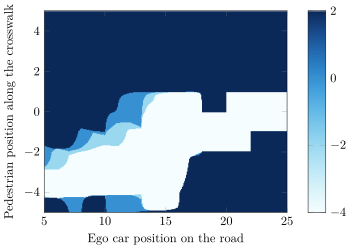
\includegraphics[width=0.5\linewidth]{src/plots/qmdp_0_00001_noise_0_01.png}
        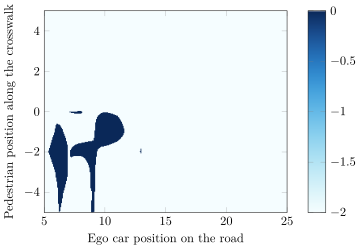
\includegraphics[width=0.5\linewidth]{src/plots/sarsop_0_01_1000_noise_0_01.png}
    }
    \caption{Policy plots for the occluded crosswalk problem with the gradations representing accelerations in $\si{\meter\per\square\second}$. There is no error in the sensing of the pedestrian's position and velocity.}
    \label{fig:qmdp_sarsop_1}
\end{figure}

The policies exhibit similar behavior, though the QMDP policy is more aggressive throughout, with aggressive braking for most of the ego vehicle's positions. The SARSOP policy appears similar, though the policy oddly switches to less aggressive braking as the ego approaches the pedestrian. This may be due to the $1000 ~\si{\second}$ time-out termination condition we set for SARSOP. The policies are topologically similar to those presented in \cite{Bouton2018ScalableDriving}.

We also, analyzed the effect of sensor uncertainty in each POMDP solver to examine the robustness to uncertainty in the environment and the sensors, which is shown in \Cref{fig:qmdp_sarsop_2}.

\begin{figure*}[htbp]
    \centerline{\textbf{QMDP Policies}}
    \centerline{
        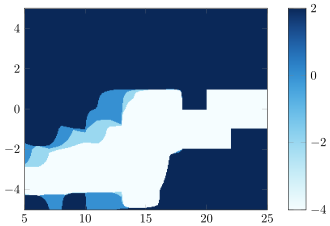
\includegraphics[width=0.25\linewidth]{src/plots/qmdp_0_00001_noise_0_01_no_labels.png}
        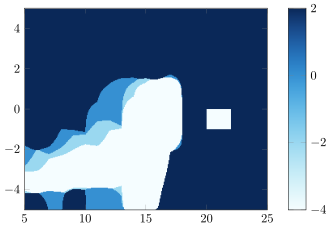
\includegraphics[width=0.25\linewidth]{src/plots/qmdp_0_00001_noise_0_5_no_labels.png}
        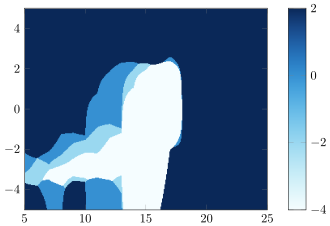
\includegraphics[width=0.25\linewidth]{src/plots/qmdp_0_00001_noise_1_0_no_labels.png} 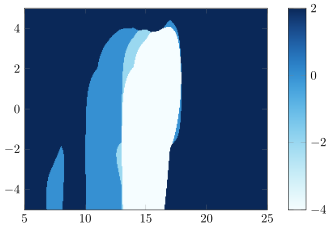
\includegraphics[width=0.25\linewidth]{src/plots/qmdp_0_00001_noise_2_0_no_labels.png}
    }
    ~ \\
    \centerline{\textbf{SARSOP Policies}}
    \centerline{
        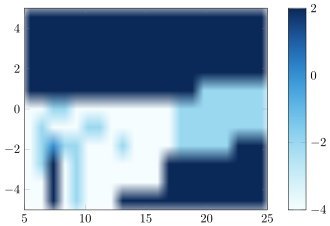
\includegraphics[width=0.25\linewidth]{src/plots/sarsop_0_01_1000_noise_0_01_no_labels.png}
        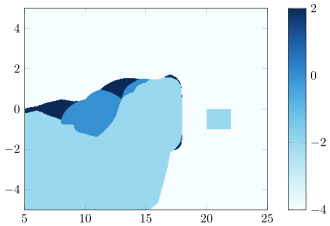
\includegraphics[width=0.25\linewidth]{src/plots/sarsop_0_01_1000_noise_05_no_labels.png}
        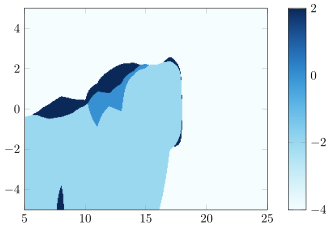
\includegraphics[width=0.25\linewidth]{src/plots/sarsop_0_01_1000_noise_10_no_labels.png} 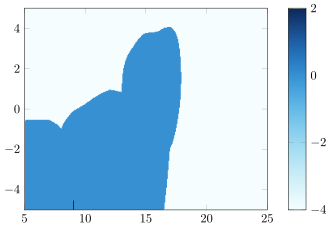
\includegraphics[width=0.25\linewidth]{src/plots/sarsop_0_01_1000_noise_20_no_labels.png}
    }
    \caption{Policy plots for the occluded crosswalk problem with the gradations representing accelerations in $\si{\meter\per\square\second}$. The horizontal axis represents the position of the ego vehicle in the roadway in $\si{\meter}$, with the right edge of the plot representing the location of the crosswalk; the vertical axis represents the position of the pedestrian in the crosswalk in $\si{\meter}$. The ego vehicle is initialized at $5 ~\si{\meter\per\second}$ and the pedestrian is initialized at $1 ~\si{\meter\per\second}$. From left to right, the standard deviation of the sensor's position and velocity estimates increases ($\sigma = 0~ \si{\meter}$, $\sigma = 0.5~ \si{\meter}$, $\sigma = 1~ \si{\meter}$, $\sigma = 2~ \si{\meter}$), demonstrating the POMDP's robustness to uncertainty.}
    \label{fig:qmdp_sarsop_2}
\end{figure*}


Following the choices of the authors in \cite{Bouton2018ScalableDriving} in order to balance safety and efficiency, we set the collision penalty for QMDP to $-1.6$ and the collision penalty for SARSOP to $-30$. The position sensor uncertainty was set to $0.5 ~\si{\meter}$ and the velocity sensor uncertainty was set to $0.5 ~\si{\meter\per\second}$.

\begin{table}[htbp]
    \caption{Results of Occluded Crosswalk Policies}
    \begin{center}
        \begin{tabular}{lrr}
            \hline \hline
             & \textbf{Collision rate} \hspace{3pt} & \textbf{Time to cross} \hspace{1pt} \\
            \hline
            \textbf{Random} & $18.65 \pm 38.95\%$ & $16.70 \pm 7.72 ~\si{\second}$ \\
            \textbf{QMDP}   & $4.00 \pm 19.69\%$  & $5.34 \pm 0.98 ~\si{\second}$ \\
            \textbf{SARSOP}\footnote{The SARSOP scenario were not finished since the belief update for SARSOP takes much longer than for SARSOP.} & -- & -- \\
            \hline \hline
        \end{tabular}
        \label{tab1}
    \end{center}
\end{table}

The random policy results were computed over 10,000 simulations, while the QMDP policy and SARSOP policy results we computed on 100 simulations, due to the increased computational cost of performing the belief update.

discussion and comparison with the results in Bouton paper

\section{Conclusion}
\label{sec:conclusion}

%In general a short summarizing paragraph will do, and under no circumstances should the paragraph simply repeat material from the Abstract or Introduction. In some cases it's possible to now make the original claims more concrete, e.g., by referring to quantitative performance results.

\section{Future Work}
\label{sec:future-work}

We will continue to investigate some of the topics presented in this paper. It would be good to get a complete comparison of the random, QMDP, and SARSOP policies' collision rates and times-to-cross, possibly with more simulations to provide tighter error bounds. Additionally, a baseline manually-designed policy based on a time-to-collision (TTC) metric would also provide meaningful results for comparison.

The policies discussed in this paper were all generated using offline methods. A future research direction is to explore online methods while avoiding discretization of state, action, and observation spaces. A first step would be to use the partially observable Monte Carlo planning (POMCP) algorithm \cite{Silver2010Monte-CarloPOMDPs} or the determinized sparse partially observable trees (DESPOT) algorithm augmented with importance sampling to include rare, but critical events \cite{Ye2017DESPOT:Regularization, Luo2019ImportanceUncertainty}. 

Beyond this the POMDP could be considered in its natural continuous form and solved with a variety of algorithms based on progressive widening (PW), namely, the partially observable Monte Carlo planning with observation widening (POMCPOW) algorithm \cite{Sunberg2018OnlineSpaces}. We expect these methods to be much more difficult to compute but possibly more efficient given the continuous nature of the state, action, and observation spaces.

It would also be interesting to see the performance of many of these policies in the presence of cyclists, who are important, but frequently neglected road users. Since cyclists typically have much higher velocities, we expect the policies learned from pedestrian behavior to fail, but future research could be done to develop hybrid policies that at least avoid a subset of cyclist collisions while maintaining or improving pedestrian safety.

\bibliographystyle{IEEEtran}
\bibliography{main}

\end{document}

